%	$Id: lhcppfront.tex,v 1.9 1999/09/07 06:56:43 goossens Exp goossens $	
%%%%%%%%%%%%%%%%%%%%%%%%%%%%%%%%%%%%%%%%%%%%%%%%%%%%%%%%%%%%%%%%%%%
%                                                                 %
%   LHC Plus Plus Latex Front matter                              %
%                                                                 %
%   Front Material: Title page,                                   %
%                   Copyright Notice                              %
%                   Preliminary Remarks                           %
%                   Table of Contents                             %
%   EPS file      : cern15.eps, cnastit.eps                       %
%                                                                 %
%   Editor: Michel Goossens / IT-ASD                              %
%                                                                 %
%%%%%%%%%%%%%%%%%%%%%%%%%%%%%%%%%%%%%%%%%%%%%%%%%%%%%%%%%%%%%%%%%%%

%%%%%%%%%%%%%%%%%%%%%%%%%%%%%%%%%%%%%%%%%%%%%%%%%%%%%%%%%%%%%%%%%%%%
%    Tile page                                                     %
%%%%%%%%%%%%%%%%%%%%%%%%%%%%%%%%%%%%%%%%%%%%%%%%%%%%%%%%%%%%%%%%%%%%
\def\Ptitle#1{\special{ps: /Printstring (#1) def}
                       \epsfbox{cnastit.eps}}
\begin{titlepage}
\vspace*{-23mm}
\includegraphics[height=30mm]{cern15.eps}%
\hfill
\raisebox{10mm}{\Large\bf CERN Computer Program Library Documentation}
\hfill\mbox{}
\begin{center}
\mbox{}\\[10mm]
\mbox{\Ptitle{LHC++}}\\[2cm]
{\Huge C++ Libraries for HEP}\\[1cm]
{\LARGE Version 2.0.1 }\\[3cm]
%{\Large DRAFT (comments welcome)}\\[2cm]
{\Large Applications for Physics & Infrastructure}\\[5mm]
{\Large Information Technologies Division}\\[2cm]
{\Large CERN Geneva, Switzerland}
\end{center}
\end{titlepage}

%%%%%%%%%%%%%%%%%%%%%%%%%%%%%%%%%%%%%%%%%%%%%%%%%%%%%%%%%%%%%%%%%%%%
%    Copyright  page                                               %
%%%%%%%%%%%%%%%%%%%%%%%%%%%%%%%%%%%%%%%%%%%%%%%%%%%%%%%%%%%%%%%%%%%%
\thispagestyle{empty}
\framebox[\textwidth][t]{\hfill\begin{minipage}{0.96\textwidth}%
\vspace*{3mm}\begin{center}Copyright Notice\end{center}
\parskip\baselineskip
\textbf{C++ Libraries for HEP}
 
CERN Program Library Documentation
 
\copyright{} Copyright CERN, Geneva 1997--1999
 
Copyright and any other appropriate legal protection of these
computer programs and associated documentation reserved in all
countries of the world by their respective copyright holders.

These programs or documentation may not be reproduced by any method
without prior written consent of the Director-General of CERN or his
delegate or from the original copyright holders for the commercial
components.
 
Requests for information should be addressed to:
\vspace*{-.5\baselineskip}
\begin{center}
\tt\begin{tabular}{l}
CERN Program Library Office              \\
CERN-IT Division                         \\
CH-1211 Geneva 23                        \\
Switzerland                              \\
Tel.   +41 22 767 4951                   \\
Fax.   +41 22 767 8630                   \\
Email: cernlib@cern.ch
\end{tabular}
\end{center}
\vspace*{2mm}
\end{minipage}\hfill}%end of minipage in framebox
\vspace{6mm} \textbf{Trademark notice: All trademarks appearing in
  this guide are acknowledged as such.}  
\vfill 
{\small The source of this document is marked up in \textsc{xml}
  using a \textsc{dtd} copied on a subset of \LaTeX's functionality.
  It is translated with an \textsc{xsl} style sheet and James
  Clark's \texttt{xt} Java program into \LaTeX{} and \textsc{html}.
  The \LaTeX{} source is further typeset using the \Lit{cernman}
  class file developed at CERN and a printable PostScript file is
  generated.}
\vfill
\begin{flushleft}
\emph{Contact Person}: Andreas Pfeiffer /IT 
                        (\texttt{Andreas.Pfeiffer@cern.ch})\\
\emph{Documentation}: Michel Goossens /IT 
                        (\texttt{michel.goossens@cern.ch})\\[5mm]
\emph{Edition -- September 1999} \hfill \footnotesize Printed \today
\end{flushleft}
\newpage

%%%%%%%%%%%%%%%%%%%%%%%%%%%%%%%%%%%%%%%%%%%%%%%%%%%%%%%%%%%%%%%%%%%%
%    Introductory material                                         %
%%%%%%%%%%%%%%%%%%%%%%%%%%%%%%%%%%%%%%%%%%%%%%%%%%%%%%%%%%%%%%%%%%%%
\pagenumbering{roman}
\setcounter{page}{1}

\section*{Preliminary remarks}
 
This manual serves at the same time as an introduction 
to the various components of LHC++ and also aims to help
you to get started with the system.

Chapter 1 briefly describes the objectives of the LHC++ Project and
describes its various components, while the LHC++ Analysis Model is
introduced in Chapter 2. Chapter 3 explains what you should do to set
up the LHC++ environment, and Chapter 4 gives a few hints about the
object database. The histogram and tag classes and their use are the
subject of Chapter 5. Finally a glossary and an index conclude this guide.

\section*{If you need help}

The LHC++ Project page is available on WWW at the URL:
\begin{center}
\fbox{\texttt{http://wwwinfo.cern.ch/asd/lhc++/index.html}}
\end{center}
The page also tells you how to subscribe to the LHC++ mailing list,
and presents a detailed list of LHC++ contact persons. 

\section*{Documentation and examples}
\label{SEC:DOCEXA}
\index{Examples!location}\index{Examples!running \~{}}%
\index{Documentation!location}%

Examples for the HTL and hepodbms packages
are available in the directories:
\begin{center}
\begin{tabular}{|ll|}\hline
Unix & \texttt{/afs/cern.ch/sw/lhcxx/share/HTL/<version>/HTL/examples}\\
     & \texttt{/afs/cern.ch/sw/lhcxx/share/HepODBMS/<version>/HepODBMS/examples}\\[1mm]
\\\hline
\end{tabular}
\end{center}
Each example has its own subdirectory, containing the C++ source code
in a file with extension \texttt{cpp}, as well as a
\texttt{GNUmakefile} which allows you to generate an executable with
\texttt{gmake}.

The \textsc{html} version of this guide can be found at the URL
\url{http://wwwinfo.cern.ch/asdoc/lhcpp/lhcpp.html}. The printable
PostScript version is also available from that page.  Alternatively,
the same PostScript file can be obtained as a gzipped compressed file
\texttt{lhcpp.ps.gz}, from any CERN machine, or any machine registered
for cernlib access, by anonymous ftp as follows (commands to be typed
by the user are underlined):

\vspace*{3mm} 
\begin{XMP}
    \underline{ftp asisftp.cern.ch}
    Connected to asis00.cern.ch.
    220 asis00 FTP server (Version wu-2.4(2)...) ready.
    Name (asisftp:username): \underline{ftp}
    Password: \underline{your\_{}mailaddress}
    230 Guest login ok, access restrictions apply.
    ftp> \underline{cd cernlib/doc/ps.dir}
    ftp> \underline{get lhcpp.ps.gz}    (type \Ucom{get lhcpp.ps} for the uncompressed version)
    ftp> \underline{quit}
\end{XMP}

%%%%%%%%%%%%%%%%%%%%%%%%%%%%%%%%%%%%%%%%%%%%%%%%%%%%%%%%%%%%%%%%%%%%
%    Tables of contents ...                                        %
%%%%%%%%%%%%%%%%%%%%%%%%%%%%%%%%%%%%%%%%%%%%%%%%%%%%%%%%%%%%%%%%%%%%
\newpage
\tableofcontents
\newpage
\listoffigures
%\listoftables
\endinput


